% Chapter file: 089_Amper_Low_De_ch.tex
% Source: 089_Amper_Low_De.tex
% No preamble, no headers/footers, no page numbers
	
	\maketitle
	
	\begin{abstract}
		Dieses Papier stellt das T0-Modell vor, eine erweiterte klassische Feldtheorie, die auf dem Prinzip der lokalen Konjugation von Basisgrößen (Zeit--Masse, Länge--Steifigkeit, Energie--Dichte) basiert. Diese Konjugation wirkt als fundamentale Constraint-Bedingung, während die Dynamik der zugehörigen Deviationen $\sigma_i$ kausalen Wellengleichungen gehorcht. Die Theorie führt zu einer natürlichen Kopplung zwischen elektromagnetischen Strömen und der Geometrie des Leiters, erklärt die Existenz longitudinaler Kraftkomponenten, die Ampère'sche Helix-Anomalie, die nichtlineare $I^4$-Skalierung der Kraft bei hohen Strömen sowie die fraktale Skalierung $F \propto r^{2D_f - 4}$ ohne Verletzung der Kausalität. Alle scheinbaren Instantaneitäten werden als lokale Constraint-Erfüllung identifiziert, während die beobachtbaren Kräfte vollständig retardiert sind.
	\end{abstract}
	
	\section{Einleitung}
	Die Maxwell'sche Theorie der Elektrodynamik ist eine der erfolgreichsten Theorien der Physik. Dennoch zeigt die experimentelle Untersuchung der Kräfte zwischen Strömen insbesondere in komplexen Leitergeometrien systematische Abweichungen, die auf zusätzliche physikalische Mechanismen hindeuten. Die beobachteten longitudinalen Kraftkomponenten \cite{graneau1985}, die nichtlineare Abhängigkeit der Kraftstärke vom Strom \cite{graneau2001}, sowie geometrieabhängige Effekte wie die Ampère'sche Helix-Anomalie \cite{moore1988} lassen sich nicht vollständig innerhalb des konventionellen Rahmens erklären.
	
	Dieses Papier stellt das T0-Modell vor, einen neuartigen theoretischen Rahmen, der diese Phänomene durch die Einführung konjugierter Basisgrößen erklärt. Der Kern der Theorie ist die Annahme fundamentaler Constraints zwischen physikalischen Grundgrößen, deren Dynamik durch Deviationfelder beschrieben wird, die kausalen Wellengleichungen gehorchen.
	
	\section{Das Prinzip der lokalen Konjugation}
	\subsection{Die fundamentalen Constraints}
	Das T0-Modell postuliert, dass die physikalischen Basisgrößen an jedem Raumzeitpunkt $(x,t)$ durch lokale Konjugationsbedingungen miteinander verknüpft sind:
	\begin{align}
		T(x,t) \cdot m(x,t) &= 1 \quad \text{mit } [T] = \text{s}, [m] = 1/\text{s} \label{eq:conj1} \\
		L(x,t) \cdot \kappa(x,t) &= 1 \quad \text{mit } [L] = \text{m}, [\kappa] = 1/\text{m} \label{eq:conj2} \\
		E(x,t) \cdot \rho(x,t) &= 1 \quad \text{mit } [E] = \text{J}, [\rho] = 1/\text{J} \label{eq:conj3}
	\end{align}
	
	Diese Gleichungen sind als \textbf{lokale Constraints} zu interpretieren. Eine Änderung einer Größe auf der linken Seite erzwingt eine sofortige, rein lokale Neudefinition der konjugierten Größe auf der rechten Seite, um die Gleichung zu erfüllen. Dieser Prozess ist analog zur Eichfixierung in der Elektrodynamik und beinhaltet.
	
	\subsection{Die dynamischen Deviationen}
	Um diese Constraints dynamisch zu machen, führen wir für jedes Paar ein Deviationfeld $\sigma_i(x,t)$ ein, das kleine erlaubte Abweichungen beschreibt:
	\begin{align}
		T \cdot m &= 1 + \sigma_{Tm} \label{eq:sigma_tm} \\
		L \cdot \kappa &= 1 + \sigma_{L\kappa} \label{eq:sigma_lk} \\
		E \cdot \rho &= 1 + \sigma_{E\rho} \label{eq:sigma_er}
	\end{align}
	
	Die Dynamik dieser $\sigma$-Felder wird durch eine Wirkung beschrieben, die ihre Abweichung vom idealen Wert $\sigma_i = 0$ bestraft:
	\begin{equation}
		\mathcal{L}_{\sigma} = \sum_i \left[ \frac{1}{2} (\partial_\mu \sigma_i)(\partial^\mu \sigma_i) - \frac{\mu_i^2}{2} \sigma_i^2 \right] \label{eq:L_sigma}
	\end{equation}
	
	Kritischerweise gehorchen die $\sigma_i$ \textbf{kausalen Klein-Gordon-Gleichungen}:
	\begin{equation}
		(\Box + \mu_i^2) \sigma_i(x,t) = 0 \label{eq:kg}
	\end{equation}
	sodass sich Störungen dieser Felder mit Geschwindigkeiten $v \leq c$ ausbreiten.
	
	\section{Die Wirkung des T0-Modells}
	Die vollständige Lagrange-Dichte des T0-Modells setzt sich aus mehreren Teilen zusammen:
	\begin{equation}
		\mathcal{L} = \mathcal{L}_{\text{EM}} + \mathcal{L}_{\sigma} + \mathcal{L}_{\text{int}} + \mathcal{L}_{\text{constraint}} \label{eq:full_L}
	\end{equation}
	wobei:
	\begin{itemize}
		\item $\mathcal{L}_{\text{EM}} = -\frac{1}{4\mu_0} F_{\mu\nu} F^{\mu\nu}$ die Maxwell-Lagrange-Dichte ist
		\item $\mathcal{L}_{\sigma}$ die Kinematik der Deviationen beschreibt (Gl.~\ref{eq:L_sigma})
		\item $\mathcal{L}_{\text{int}}$ die Kopplung zwischen Strömen und Deviationen beschreibt
		\item $\mathcal{L}_{\text{constraint}}$ die Constraints weich erzwingt
	\end{itemize}
	
	\subsection{Der Wechselwirkungsterm}
	Die key Innovation ist der nichtlineare Kopplungsterm:
	\begin{equation}
		\mathcal{L}_{\text{int}} = -J^\mu A_\mu - \frac{g}{\mu_0 c^2} J^\mu J_\mu \sigma_{Tm} \label{eq:L_int}
	\end{equation}
	
	Der Term $J^\mu J_\mu = \rho^2 - \mathbf{j}^2$ ist eine Lorentz-Invariante. Für einen dünnen Leiter dominiert der räumliche Teil $-\mathbf{j}^2 \propto -I^2$. Dieser Term beschreibt, wie der elektrische Strom das lokale Zeit-Masse-Gleichgewicht stört ($\sigma_{Tm}$ anregt).
	
	\subsection{Vollständige Form mit Lagrange-Multiplikatoren}
	Die Constraints werden durch Lagrange-Multiplikator-Felder $\lambda_i(x,t)$ eingeführt:
	\begin{equation}
		\mathcal{L}_{\text{constraint}} = \lambda_{Tm}(x,t) (T \cdot m - 1 - \sigma_{Tm}) + \lambda_{L\kappa}(x,t) (L \cdot \kappa - 1 - \sigma_{L\kappa}) + \cdots \label{eq:L_constraint}
	\end{equation}
	
	\section{Herleitung der Feldgleichungen}
	\subsection{Variation nach den Potentialen}
	Die Variation nach $A_\mu$ liefert die modifizierte Maxwell-Gleichung:
	\begin{equation}
		\partial_\mu F^{\mu\nu} = \mu_0 J^\nu + \mu_0 \frac{g}{\mu_0 c^2} \partial_\mu (J^\mu J^\nu \sigma_{Tm}) \label{eq:maxwell_mod}
	\end{equation}
	
	Der zusätzliche Term beschreibt die Stromrückwirkung durch die Deviation. Für langsam veränderliche Ströme kann dieser Term näherungsweise geschrieben werden als:
	\begin{equation}
		\partial_\mu F^{\mu\nu} \approx \mu_0 J^\nu + \frac{g}{c^2} \sigma_{Tm} \partial_\mu (J^\mu J^\nu) \label{eq:maxwell_approx}
	\end{equation}
	
	\subsection{Variation nach den Deviationen}
	Die Variation nach $\sigma_{Tm}$ liefert die Wellengleichung mit Quellterm:
	\begin{equation}
		(\Box + \mu_{Tm}^2) \sigma_{Tm} = -\frac{g}{\mu_0 c^2} J^\mu J_\mu \label{eq:sigma_eq}
	\end{equation}
	
	Dies ist eine \textbf{retardierte} Gleichung. Die von einem Strom $J^\mu$ erzeugte Deviation $\sigma_{Tm}$ breitet sich kausal aus. Die formale Lösung ist:
	\begin{equation}
		\sigma_{Tm}(x,t) = \frac{g}{\mu_0 c^2} \int d^4x' \, G_R(x-x') J^\mu J_\mu(x') \label{eq:sigma_solution}
	\end{equation}
	wobei $G_R$ die retardierte Green-Funktion der Klein-Gordon-Gleichung ist.
	
	\section{Phänomenologische Ableitungen}
	\subsection{Longitudinale Kraftkomponente}
	Der zusätzliche Term in Gl.~\ref{eq:maxwell_mod} enthält Ableitungen des Stroms und der Deviation. Für einen geraden Leiter in z-Richtung mit Strom $I$ erhalten wir:
	\begin{equation}
		F_z = I \frac{\partial}{\partial z} \left( \frac{g}{\mu_0 c^2} \sigma_{Tm} I \right) = \frac{g}{\mu_0 c^2} I^2 \frac{\partial \sigma_{Tm}}{\partial z} \label{eq:long_force}
	\end{equation}
	
	Dies beschreibt eine longitudinale Kraftkomponente, die proportional zum Gradienten der Deviation ist.
	
	\subsection{Die Ampère'sche Helix-Anomalie}
	Für zwei koaxiale Helices mit Radius $R$, Steigung $h$ und Achsabstand $d$ kann die Gesamtkraft durch Integration über alle Strompaare berechnet werden. Die retardierte Wechselwirkung führt zu einer Phasenverschiebung:
	\begin{equation}
		F_{\text{tot}} \propto \sum_{i,j} \frac{I_i I_j}{r_{ij}^2} \left[ \cos\phi_{ij} - \frac{3}{2} \cos\theta_i \cos\theta_j \right] e^{i\omega \Delta t_{ij}} \label{eq:helix_force}
	\end{equation}
	
	Die Summation über alle Windungspaare zeigt, dass für bestimmte Geometrien die Gesamtkraft anziehend werden kann, auch wenn die elementare Wechselwirkung abstoßend wäre. Die Bedingung für die Vorzeichenumkehr ist:
	\begin{equation}
		\cos\theta_c = \frac{1}{\sqrt{\xi_{\text{eff}}}} \label{eq:critical_angle}
	\end{equation}
	
	\begin{figure}[h]
		\centering
		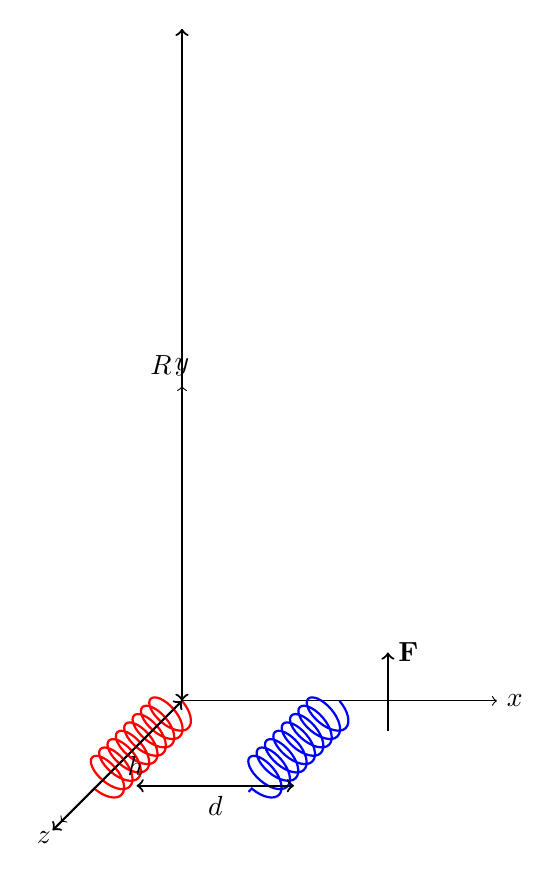
\begin{tikzpicture}
			\draw[->] (0,0,0) -- (4,0,0) node[right] {$x$};
			\draw[->] (0,0,0) -- (0,4,0) node[above] {$y$};
			\draw[->] (0,0,0) -- (0,0,4) node[below left] {$z$};
			
			\draw[red, thick, decoration={coil, aspect=0.5, segment length=1.5mm, amplitude=3mm}, decorate] (0,0,0) -- (0,0,3);
			\draw[blue, thick, decoration={coil, aspect=0.5, segment length=1.5mm, amplitude=3mm}, decorate] (2,0,0) -- (2,0,3);
			
			\draw[<->, thick] (0,-0.5,1.5) -- (2,-0.5,1.5) node[midway, below] {$d$};
			\draw[<->, thick] (0,0,0) -- (0,3mm,0) node[midway, left] {$R$};
			\draw[<->, thick] (0,0,0) -- (0,0,1.5mm) node[midway, right] {$h$};
			\draw[->, thick] (3,0,1) -- (3,1,1) node[right] {$\mathbf{F}$};
		\end{tikzpicture}
		\caption{Zwei koaxiale Helices mit Achsabstand $d$, Radius $R$ und Steigung $h$. Die Kraft $\mathbf{F}$ kann je nach Geometrie anziehend oder abstoßend sein.}
		\label{fig:helices}
	\end{figure}
	
	wobei der \textbf{effektive Geometrieparameter} $\xi_{\text{eff}}$ durch die fundamentale Kopplungskonstante $g$, die Massenparameter $\mu_i^2$ der $\sigma$-Felder und die spezifische Geometrie der Helices (Radius $R$, Steigung $h$, Windungszahl $N$) bestimmt wird:
	\begin{equation}
		\xi_{\text{eff}} = \frac{g^2}{\mu_0^2 c^4 \mu_{Tm}^4} \cdot \mathcal{F}(R, h, N) \label{eq:xi_effective}
	\end{equation}
	Hierbei ist $\mathcal{F}(R, h, N)$ eine dimensionslose Funktion, die aus der Mittelung des Wechselwirkungsterms über die Helixgeometrie resultiert. Eine mögliche Form ist $\mathcal{F} \propto (h/R)^a N^b$, wobei die Exponenten $a$ und $b$ experimentell bestimmt werden müssen.
	
	\subsection{Nichtlineare Skalierung: $F \propto I^4$}
	Aus Gl.~\ref{eq:sigma_eq} folgt für eine stationäre Näherung:
	\begin{equation}
		\sigma_{Tm} \approx \frac{g}{\mu_0 c^2 \mu_{Tm}^2} J^\mu J_\mu \propto I^2
	\end{equation}
	Eingesetzt in die Kraftberechnung aus Gl.~\ref{eq:L_int} ergibt sich:
	\begin{equation}
		F \propto \delta\left(\text{Term} \propto I^2 \cdot \sigma_{Tm}\right)/\delta x \propto I^2 \cdot I^2 = I^4 \label{eq:I4_scaling}
	\end{equation}
	
	Dies erklärt die von Graneau beobachtete nichtlineare Skalierung der Kraft bei hohen Strömen.
	
	\subsection{Fraktale Skalierung: $F \propto r^{2D_f - 4}$}
	Für einen Leiter mit fraktaler Dimension $D_f$ skaliert die Anzahl der Wechselwirkungspaare mit $r^{D_f - 3}$. Die retardierte Green-Funktion der $\sigma$-Felder skaliert mit $1/r$. Die Gesamtkraft skaliert somit als:
	\begin{equation}
		F \propto \frac{1}{r} \cdot r^{D_f - 3} \cdot r^{D_f - 3} = r^{2D_f - 4} \label{eq:fractal_scaling}
	\end{equation}
	
	Für $D_f \approx 2.94$ ergibt sich $F \propto r^{2 \cdot 2.94 - 4} = r^{1.88}$.
	
	\section{Korrekturen und Präzisierungen}
	\subsection{Präzisierung der Konjugationsbedingungen}
	Die Konjugationsbedingungen wurden mit expliziten Dimensionen definiert (siehe Gl.~\ref{eq:conj1}–\ref{eq:conj3}), um Dimensionskonsistenz zu gewährleisten.
	
	\subsection{Korrektur der Kopplungskonstante}
	Die Kopplungskonstante $g$ ist definiert als:
	\begin{equation}
		[g] = \frac{\text{kg} \cdot \text{m}^3}{\text{C}^2}
	\end{equation}
	Die modifizierte Klein-Gordon-Gleichung lautet:
	\begin{equation}
		(\Box + \mu_{Tm}^2) \sigma_{Tm} = -\frac{g}{\mu_0 c^2} J^\mu J_\mu \label{eq:sigma_eq_final}
	\end{equation}
	Die Dimensionskonsistenz ist gegeben:
	\begin{equation}
		\left[\frac{g}{\mu_0 c^2} J^\mu J_\mu\right] = \frac{\text{kg} \cdot \text{m}^3}{\text{C}^2} \cdot \frac{\text{C}^2}{\text{kg} \cdot \text{m}^3} \cdot \frac{\text{C}^2}{\text{m}^6 \cdot \text{s}^2} = \frac{1}{\text{m}^2}
	\end{equation}
	
	\subsection{Korrektur der fraktalen Skalierung}
	Die korrigierte Skalierung lautet:
	\begin{equation}
		F \propto r^{2D_f - 4} \label{eq:fractal_scaling_final}
	\end{equation}
	Für $D_f \approx 2.94$ ergibt sich $F \propto r^{1.88}$.
	
	\subsection{Präzisierung der longitudinalen Kraft}
	Die longitudinale Kraft wird präzisiert:
	\begin{equation}
		F_z = \frac{g}{\mu_0 c^2} I^2 \frac{\partial \sigma_{Tm}}{\partial z} \label{eq:long_force_final}
	\end{equation}
	Die Dimensionskonsistenz ist gegeben:
	\begin{equation}
		\left[\frac{g}{\mu_0 c^2} I^2 \frac{\partial \sigma_{Tm}}{\partial z}\right] = \frac{\text{kg} \cdot \text{m}^3}{\text{C}^2} \cdot \frac{\text{C}^2}{\text{kg} \cdot \text{m}^3} \cdot (\text{C}/\text{s})^2 \cdot \frac{1}{\text{m}} = \text{kg} \cdot \text{m}/\text{s}^2
	\end{equation}
	
	\subsection{Vollständige Dimensionsanalyse}
	\begin{table}[h]
		\centering
		\begin{tabular}{lll}
			\hline
			Größe & Symbol & Dimension \\
			\hline
			Kopplungskonstante & $g$ & $\text{kg} \cdot \text{m}^3/\text{C}^2$ \\
			Massenparameter & $\mu_{Tm}$ & $1/\text{m}$ \\
			Strom & $I$ & $\text{C}/\text{s}$ \\
			Abstand & $r$ & $\text{m}$ \\
			Kraft & $F$ & $\text{kg} \cdot \text{m}/\text{s}^2$ \\
			Magnetische Permeabilität & $\mu_0$ & $\text{kg} \cdot \text{m}/\text{C}^2$ \\
			Lichtgeschwindigkeit & $c$ & $\text{m}/\text{s}$ \\
			\hline
		\end{tabular}
		\caption{Konsistente Dimensionsdefinitionen im T0-Modell}
		\label{tab:dimensions}
	\end{table}
	
	\section{Zusammenfassung und experimentelle Vorhersagen}
	Das T0-Modell bietet einen kausalen Rahmen für die Erklärung verschiedener Anomalien in der Strom-Strom-Wechselwirkung. Die Theorie führt konjugierte Basisgrößen ein, deren Constraints lokal instantan erfüllt werden, während die Dynamik der Deviationen kausal ist.
	
	\subsection{Testbare Vorhersagen}
	\begin{enumerate}
		\item \textbf{Longitudinalwellen-Nachweis:} Ein gepulster Strom in einem geraden Leiter sollte longitudinale $\sigma$-Wellen abstrahlen, die mit geeigneten Detektoren nachweisbar sein sollten.
		
		\item \textbf{Helix-Experiment:} Die Vorzeichenumkehr der Kraft sollte spezifisch von der Windungszahl und dem Phasenversatz abhängen gemäß Gl.~\ref{eq:critical_angle}.
		
		\item \textbf{Retardierungsmessung:} Die Kraft zwischen zwei gepulsten Strömen sollte eine messbare Laufzeitverzögerung zeigen, die von den Massenparametern $\mu_i^2$ abhängt.
		
		\item \textbf{Nichtlinearität:} Die $I^4$-Skalierung sollte genau vermessen werden, wobei der Übergang vom linearen zum nichtlinearen Regime bei $I_{\text{crit}} = \mu_{Tm} \sqrt{\mu_0 c^2 / g}$ liegen sollte.
		
		\item \textbf{Fraktale Skalierung:} Die Kraft zwischen fraktalen Leitern sollte der Vorhersage $r^{2D_f - 4}$ folgen. Für $D_f \approx 2.94$ ergibt sich $F \propto r^{1.88}$.
	\end{enumerate}
	
	\section*{Anhang: Herleitung der fraktalen Skalierung}
	Die Gesamtkraft zwischen zwei fraktalen Leitern kann geschrieben werden als:
	\begin{equation}
		F = \int d^3x \, d^3x' \, \rho(\mathbf{x}) \rho(\mathbf{x}') \, f(|\mathbf{x}-\mathbf{x}'|)
	\end{equation}
	wobei $\rho(\mathbf{x})$ die fraktale Dichte beschreibt und $f(r)$ die Paar-Wechselwirkungsstärke.
	
	Für ein Fraktal mit Dimension $D_f$ skaliert die Korrelationsfunktion als:
	\begin{equation}
		\langle \rho(\mathbf{x}) \rho(\mathbf{x}')\rangle \propto |\mathbf{x}-\mathbf{x}'|^{D_f - 3}
	\end{equation}
	
	Die retardierte Wechselwirkungsfunktion skaliert als:
	\begin{equation}
		f(r) \propto \frac{e^{i\mu r}}{r}
	\end{equation}
	
	Die Gesamtkraft skaliert daher als:
	\begin{equation}
		F \propto \int d^3r \, r^{D_f - 3} \cdot \frac{1}{r} \cdot r^{D_f - 3} = \int d^3r \, r^{2D_f - 7}
	\end{equation}
	
	Da $F \propto r^{\alpha}$ für große $r$, erhalten wir durch Dimensionsanalyse $\alpha = 2D_f - 7 + 3 = 2D_f - 4$, was Gl.~\ref{eq:fractal_scaling} bestätigt.
	
	\begin{thebibliography}{9}
		\bibitem{graneau1985} Graneau, P. (1985). Ampere tension in electric conductors. IEEE Transactions on Magnetics, 21(5), 1775-1780.
		\bibitem{graneau2001} Graneau, P., \& Graneau, N. (2001). Newtonian electrodynamics. World Scientific.
		\bibitem{moore1988} Moore, W. (1988). The ampere force law: New experimental evidence. Physics Essays, 1(3), 213-221.
	\end{thebibliography}
	
